\SourceLeaf{362}
\Needspace{24\baselineskip}
\Article{7}
The first method now gives the following result:
\[
\begin{aligned}
4\text{ decident}={}&\mathrm{I}\quad\Sigma\varepsilon\text{ from all}\\
&\phantom{\mathrm{I}\quad}{-}4\Sigma\varepsilon\text{ from those where }y\text{ integer }[x]\text{ even}\\[3pt]
&\mathrm{II.}\ {-}\Sigma\varepsilon\text{ from all}\\
&\phantom{\mathrm{II.}\ }{+}4\Sigma\varepsilon\text{ from those where }[x]\text{ even }[y]\text{ odd}\\[3pt]
&\mathrm{IV.}\ {+}4\Sigma\varepsilon\text{ from those where not both}\\
&\phantom{\mathrm{IV.}\ {+}4\Sigma\varepsilon\text{ from those where }}[x]\text{ and }[y]\text{ even}\\
&\phantom{\mathrm{IV.}\ }{+}Q
\end{aligned}
\]

Here
\[
\begin{array}{cc|l}
\text{for }A&B&Q=\\
+&+&-\text{Intens.}\ {+}\mu\omega i+\text{Int.}\ \frac12m-\mu\omega\\
+&-&-\text{Intens.}\ {+}\mu\omega+\text{Int.}\ \frac12mi-\mu\omega i\\
-&-&-\text{Intens.}\ {-}\mu\omega i-\text{Int.}\ \frac12m+\mu\omega\\
-&+&-\text{Intens.}\ {-}\mu\omega-\text{Int.}\ \frac12mi+\mu\omega i
\end{array}
\]
The following table represents this:

\[
\setlength{\arraycolsep}{4pt}
\begin{array}{cc|rr|rr|rr|rr}
\alpha&\beta& A&B&A&B&A&B&A&B\\
&&+&+&+&-&-&-&-&+\\ \cline{3-10}
+&+&+2&0&0&+2&-3&-5&-3&-5\\
+&-&0&+2&-2&0&-5&-3&-1&-3\\
-&-&-3&-1&-1&+1&-4&-2&0&-2\\
-&+&+1&-1&-1&+1&0&-2&-4&-6\\[3pt]
\multicolumn{2}{r}{\dfrac{m-1}{2}}&\text{even,}&\text{odd}&\multicolumn{6}{c}{}
\end{array}
\]

The first part of
\[
2Q\dotstwo -3-(\alpha\beta AB)+(A\alpha)+(A\beta)+(B\alpha)-(B\beta)
\]
The whole $2Q$ for
\[
\begin{aligned}
\frac{m-1}{2}\text{ odd}\quad&-3+4(A)-(B)-(\beta)+(\alpha A)+(\alpha B)\\
&\quad +(\beta A)-(\beta B)-(\alpha\beta AB)\\[3pt]
\frac{m-1}{2}\text{ even}\quad&-3+2(A)+(B)+(\beta)+(\alpha A)+(\alpha B)\\
&\quad +(\beta A)-(\beta B)+2(\beta AB)-(\alpha\beta AB)
\end{aligned}
\]

\SourceLeaf{363}
\Needspace{30\baselineskip}
Example
\[
\begin{array}{r|r}
m=+3-2i&13\\
M=-1-6i&37
\end{array}
\qquad
\begin{gathered}
(1+i)M+(-2+i)m=1\\
mM=-15-16i
\end{gathered}
\]
\[
\mu=+9+20i
\]

\[
\begin{array}{r|r|r|r}
+4+13i&+38+31i&+1&-1\\
+5+7i&+29+11i&0&+0\\
+6+i&+20-9i&0-i&-3\\
+10+14i&+58+22i&+1&+1\\
+11+8i&+49+2i&+1&-1\\
+12+2i&+40-18i&+1-i&+2\\
+16+15i&+78+13i&+2&-0\\
+17+9i&+69-7i&+1-i&+2\\
+18+3i&+60-27i&+1-i&-2\\ \cline{3-4}
\multicolumn{2}{c}{}&\multicolumn{2}{c}{\text{decident}=-2}
\end{array}
\]
\[
\begin{array}{lrr}
\mathrm{I}\dotstwo&+1&0\\
\mathrm{II}\dotstwo&0&-4\\
\mathrm{IV}\dotstwo&&0\\
Q=&-5&\\ \hline
\multicolumn{3}{c}{-8}\\
\multicolumn{3}{c}{\text{Good.}}
\end{array}
\]

\noindent I
\[
\begin{array}{r|r|r|r|r|r|r}
x&X&20\xi&20\eta&20y&20Y&\varepsilon\\
+1&0&6&1&-9&-37&-1\\
&+1&4&4&+4&-28&-1\\
&+2&2&7&+17&-19&-1\\
+2&+1&10&5&-5&-65&-1\\
&+2&8&8&+8&-56&+1\\
\multicolumn{6}{c}{}&-3
\end{array}
\]
\[
\begin{array}{r|r|r|r|r|r|r}
y&Y&20\xi&20\eta&20x&20X&\varepsilon\\
0&-1&3&2&+13&+9&+1^{*}\\
&-2&6&4&+26&+18&+1\\
&-3&9&6&+39&+27&+1\\
+1&-1&2&8&+22&+46&+1\\
\multicolumn{6}{c}{}&+4\\
\multicolumn{6}{c}{}&(+1)
\end{array}
\]

\[
\begin{array}{r|r|r|r|r|r|r}
y&X&9\xi&9\eta&9x&9Y&\varepsilon\\
0&+1&3&2&+13&-20&+1\\
-2&+2&0&3&+6&-3&-1^{*}\\
\multicolumn{6}{c}{}&0(-1)
\end{array}
\]
\[
\begin{array}{r|r|r|r|r|r|r}
x&Y&9\xi&9\eta&9y&9X&\varepsilon\\
+1&-1&1&3&+7&+17&-1\\
+2&-3&4&3&+1&+14&+1\\
\multicolumn{6}{c}{}&0
\end{array}
\]
\[
\mathrm{I}\pdot\pdot\pdot\;+1(0)
\]

\noindent II
\[
\begin{array}{r|r|l|r|r|r}
Y&6\xi&6x&6y&6X&\varepsilon\\
-1&+1&+3+9\omega&-2&-1&-1^{*}\\
-2&+2&+6+9\omega&-4&-2&+1\\
\multicolumn{5}{c}{}&0(-1)
\end{array}
\]
\noindent III
\[
\begin{array}{r|r|r|r|l|r}
x&3\xi&3y&3X&3Y&\varepsilon\\
+1&1&-2&-1&-6+9\omega&-1
\end{array}
\]

\noindent IV
\[
\begin{array}{r|r|l|r|r|r}
X&12\eta&12x&12y&12Y&\varepsilon\\
0&+1&+20+20\omega&-9&-37&-1^{*}\\
+1&+3&+24+20\omega&-3&-39&+1^{*}\\
+2&+5&+28+20\omega&+3&-41&-1\\
\multicolumn{5}{c}{}&-1(0)
\end{array}
\]
\noindent V
\[
\begin{array}{r|r|r|l|r|r}
x&4\eta&4y&4X&4Y&\varepsilon\\
+2&+1&-1&+4-20\omega&-13&+1
\end{array}
\]
\[
\begin{array}{r|r|r|r|r|r}
y&6\eta&6x&6X&6Y&\varepsilon\\
0&+2&+13&+9&-20&+1
\end{array}
\]

\SourceLeaf{364}
\Article{8}
We now wish to examine the result of I more closely. There are four combinations:\par
\noindent $1^0$, when $x$ and $X$ are integers. Here
\[
\begin{aligned}
\beta\xi&=-Bx+bX\\
\beta\eta&=-Ax+aX\\
\beta y&=-\alpha x+dX\\
\beta Y&=-Dx+\alpha X
\end{aligned}
\]

\Needspace{20\baselineskip}
Let $y^0$ and $Y^0$ be the absolutely least residues of $-\alpha x+dX$, $-Dx+\alpha X$ modulo $\beta$, and $\beta y=\beta y'+y^0$, $\beta Y=\beta Y'+Y^0$, and put
\[
\begin{alignedat}{2}
\beta u&=-By^0+bY^0\qquad&y^0&=+au-bt\\
\beta t&=-Ay^0+aY^0&Y^0&=+Au-Bt
\end{alignedat}
\]
Then $t,u$ will be integers, namely
\[
\begin{aligned}
-u+ti&=M(x+y'i)-m(X+Y'i)\;{}^*\\
i(t+ui)&=Mi(y'-y)-mi(Y'-Y)
\end{aligned}
\]

and then $\varepsilon=-1$ when\par
\noindent $t+u$ is even, $\beta,y^0,Y^0$ positive, or when two or none of the conditions holds; otherwise $\varepsilon=+1$.\par
\Needspace{22\baselineskip}
We put
\[
\begin{array}{rl}
t+ui=+\theta&\text{when }y^0\text{ and }Y^0\text{ both positive}\\
-\theta&y^0\text{ and }Y^0\text{ both negative}\\
+\theta'&y^0\text{ positive }Y^0\text{ negative}\\
-\theta'&y^0\text{ negative }Y^0\text{ positive}
\end{array}
\]
\[
\begin{array}{llr}
\text{to each divisible by }1+i\text{}&\theta&\text{there then corresponds }\varepsilon=-1\\
\text{to each divisible by }1+i\text{}&\theta'&\varepsilon=+1\\
\text{to each not divisible by }1+i\text{}&\theta&\varepsilon=+1\\
\text{to each not divisible by }1+i\text{}&\theta'&\varepsilon=-1
\end{array}
\]
provided that $\beta$ is positive.\par
For negative $\beta$ the rule is reversed.

\SourceLeaf{365}
\[
\setlength{\arraycolsep}{4pt}
\begin{array}{r|r|r|r|r|r|r|r}
x&X&y^0&Y^0&t+ui&\theta&\theta'&\varepsilon\\
+1&0&-9&+3&0-3i&&0+3i&-1\\
&+1&+4&-8&-1+2i&&-1+2i&-1\\
&+2&-3&+1&0-i&&0+i&-1\\
+2&+1&-5&-5&-1-i&+1+i&&-1\\
&+2&+8&+4&+1+2i&+1+2i&&+1
\end{array}
\]

\Article{9}
$2^0$, when $y$ and $Y$ are integers. Here let $x',X'$ be the nearest integers to $x$ and $X$, and
\[
x-x'=\frac{x^0}{\beta},\quad X-X'=\frac{X^0}{\beta}
\]
and put
\[
\begin{gathered}
\beta(t+ui)=-Mx^0+mX^0=-Mp^0+mP^0,\\
t+ui=Mp'-mP'
\end{gathered}
\]
that is,
\[
\begin{alignedat}{2}
\beta t&=-Ax^0+aX^0\qquad&x^0&=-bt+au\\
\beta u&=-Bx^0+bX^0&X^0&=-Bt+Au
\end{alignedat}
\]

Then
\[
\begin{aligned}
\varepsilon=-1,&\text{ when }\beta\text{ positive, }x^0\text{ positive, }X^0\text{ positive, }t+u\text{ even}\\
&\text{etc.}
\end{aligned}
\]
We put
\[
\begin{array}{rll}
&&\textit{better}\\
t+ui=+\theta&\text{when }x^0\text{ and }X^0\text{ positive}&+\theta''\\
=-\theta&\text{when both negative}&-\theta''\\
=+\theta'&\text{when }x^0\text{ positive, }X^0\text{ negative}&-\theta\\
=-\theta'&\text{when }x^0\text{ negative, }X^0\text{ positive}&+\theta
\end{array}
\]
where the same rule for $\varepsilon$ will hold as above.

\[
\setlength{\arraycolsep}{4pt}
\begin{array}{r|r|r|r|r|r|r|r}
y&Y&x^0&X^0&t+ui&\theta&\theta'&\varepsilon\\
0&-1&-7&+9&+1-3i&&-1+3i&+1\\
&-2&+6&-2&0+2i&&0+2i&+1\\
&-3&-1&+7&+1-i&&-1+i&+1\\
+1&-1&+2&+6&+1&+1&&+1
\end{array}
\]

\SourceLeaf{366}
It can now be proved
\begin{enumerate}\renewcommand{\labelenumi}{\arabic{enumi})}
\item That all $\theta$ obtained from (1) and from (2) are distinct from one another. Call their collection $\Theta$.
\item That all $\theta=T+Ui$ have the property that
\[
\begin{gathered}
-bT+aU\\
-BT+AU
\end{gathered}
\]
are positive numbers less than $\frac12\beta$.
\item That if $T,U$ are two integers satisfying the conditions just mentioned, $T+Ui$ is certainly in $\Theta$.\par
(How, then? It is based on the above equation $^*$.)
\item The same holds in a similar way for $\theta'$, whose collection $\Theta'$ will consist of those numbers $T'+U'i$ for which
\[
\begin{gathered}
-bT'+aU'\\
-(-BT'+AU')
\end{gathered}
\]
are positive numbers less than $\frac12\beta$.
\end{enumerate}

In our case
\[
\setlength{\arraycolsep}{4pt}
\begin{array}{r|r||r|r||r|r||r|r}
\theta&\varepsilon&\theta'&\varepsilon&\theta''&\varepsilon&\theta'''&\varepsilon\\
+1&+1&0+i&-1&+2-i&+1&+1&-1\\
+1+i&-1&0+2i&+1&+3-i&-1&+2&+1\\
+1+2i&+1&0+3i&-1&\multicolumn{4}{c}{}\\
\multicolumn{2}{c||}{}&-1+i&+1&\multicolumn{4}{c}{}\\
\multicolumn{2}{c||}{}&-1+2i&-1&\multicolumn{4}{c}{}\\
\multicolumn{2}{c||}{}&-1+3i&+1&\multicolumn{4}{c}{}
\end{array}
\]

Here
\[
\begin{aligned}
\theta&=-{}_*M+{}_*m\\
\theta'&=-{}_*M-{}_*m\\
\theta''&=+{}_*Mi+{}_*m\\
\theta'''&=+{}_*Mi-{}_*m
\end{aligned}
\]

\SourceLeaf{367}
\Article{10}
$3^0$. $y$ and $X$ integers. Let $x',Y'$ be the nearest integers to $x$ and $Y$, and
\[
x'+yi=p',\quad X+Y'i=P';\quad p-p'=\frac{p^0}{\alpha},\quad P-P'=\frac{P^0}{\alpha}
\]
and put
\[
\begin{aligned}
i(t+ui)&=Mp'-mP'=-\frac{Mp^0}{\alpha}+\frac{mP^0}{\alpha}\\
&=-\frac{Mx^0}{\alpha}+\frac{miY^0}{\alpha}\quad\text{that is}
\end{aligned}
\]
\[
\begin{alignedat}{3}
\alpha t&=-Bx^0+aY^0\quad&\text{then}\quad&x^0&=-bt+au\\
\alpha u&=+Ax^0+bY^0&&Y^0&=+At+Bu
\end{alignedat}
\]

Then
\[
\varepsilon=-1,\text{ when }\alpha\text{ positive, }x^0\text{ positive, }Y^0\text{ positive, }t+u\text{ even etc.}
\]
\Needspace{22\baselineskip}
We put
\[
\begin{array}{rll}
&&\textit{better}\\
t+ui=+\theta''&\text{when }x^0\text{ positive, }Y^0\text{ positive}&+\theta'\\
=+\theta'''&\text{when }x^0\text{ positive, }Y^0\text{ negative}&-\theta'''\\
-\theta''&\text{when }x^0\text{ negative, }Y^0\text{ negative}&-\theta'\\
-\theta'''&\text{when }x^0\text{ negative, }Y^0\text{ positive}&+\theta'''
\end{array}
\]
\[
\begin{array}{lr}
\text{Thus, for each}&\theta''\pdot\pdot\pdot\;\varepsilon=-1\\
&\theta'''\pdot\pdot\pdot\;\varepsilon=+1
\end{array}
\]
provided that $\theta''$ or $\theta'''$ is divisible by $1+i$ and $\alpha$ is positive.

\[
\setlength{\arraycolsep}{4pt}
\begin{array}{r|r|r|r|r|r|r|r}
y&X&x^0&X^0&t+ui&\theta''&\theta'''&\varepsilon\\
0&+1&+4&-2&+2&&+2&+1\\
+1&+2&-3&-3&-3+i&+3-i&&-1
\end{array}
\]

\Needspace{28\baselineskip}
\Article{11}
Class $4$, $x$ and $Y$ integers. With assumptions similar to those in 3, put
\[
\begin{aligned}
-(t+ui)&=Mp'-mP'=-\frac{Mp^0}{\alpha}+\frac{mP^0}{\alpha}\\
&=-\frac{Miy^0}{\alpha}+\frac{mX^0}{\alpha}
\end{aligned}
\]
\[
\begin{alignedat}{2}
\alpha t&=-By^0-aX^0\qquad&y^0&=-bt+au\\
\alpha u&=+Ay^0-bX^0&X^0&=-At-Bu
\end{alignedat}
\]
Then
\[
\varepsilon=+1\text{ when }\alpha\text{ positive, }y^0\text{ positive, }X^0\text{ positive, }t+u\text{ even etc.}
\]

\SourceLeaf{368}
We put
\[
\begin{array}{rl}
t+ui=+\theta''&\text{when }y^0\text{ positive }X^0\text{ negative}\\
+\theta'''&\text{when }y^0\text{ positive }X^0\text{ positive}\\
-\theta''&\text{when }y^0\text{ negative }X^0\text{ positive}\\
-\theta'''&\text{when }y^0\text{ negative }X^0\text{ negative}
\end{array}
\]
For $\varepsilon$ the rule then holds (as above in 3), provided that $\alpha$ is positive:
\[
\begin{aligned}
\varepsilon=-1\text{ for each (divisibility by }1+i\text{): }&\left\{\begin{array}{ll}\text{divisible}&\theta''\\\text{not divisible}&\theta'''\end{array}\right.\\[3pt]
\varepsilon=+1\text{ for each (divisibility by }1-i\text{): }&\left\{\begin{array}{ll}\text{divisible}&\theta'''\\\text{not divisible}&\theta''\end{array}\right.
\end{aligned}
\]

\[
\setlength{\arraycolsep}{4pt}
\begin{array}{r|r|r|r|r|r|r|r}
x&Y&y^0&X^0&t+ui&\theta''&\theta'''&\varepsilon\\
+1&-1&-2&-1&-1&&+1&-1\\
+2&-3&+1&-4&+2-i&+2-i&&+1
\end{array}
\]

The collection of all $\theta''$ from 3 and 4, which we denote by $\Theta''$, therefore consists of all numbers $T+Ui$ for which
\[
\left.\begin{array}{r}
-bT+aU\\
\text{and }+AT+BU
\end{array}\right\}\text{ positive and less than }\frac12\alpha
\]
the collection of all $\theta'''\pdot\pdot\pdot\;(\Theta''')$ of those for which
\[
\left.\begin{array}{r}
-bT+aU\\
-AT-BU
\end{array}\right\}\text{ positive and less than }\frac12\alpha
\]

\Needspace{36\baselineskip}
\Article{12}
After the above improvement, the rule therefore reads as follows:\par
Let
\[
\begin{aligned}
\Theta\quad&\text{contain all numbers }T+Ui,\text{ where }+bT-aU\text{ positive}\\
&\quad -BT+AU\text{ positive and }<\tfrac12\beta\\
\Theta'\quad&\text{contain all numbers }T+Ui,\text{ where }-bT+aU\text{ positive}\\
&\quad +AT+BU\text{ positive and }<\tfrac12\alpha\\
\Theta''\quad&\text{contain all numbers }T+Ui,\text{ where }-bT+aU\text{ positive}\\
&\quad -BT+AU\text{ positive and }<\tfrac12\beta\\
\Theta'''\quad&\text{contain all numbers }T+Ui,\text{ where }+bT-aU\text{ positive}\\
&\quad +AT+BU\text{ positive and }<\tfrac12\alpha
\end{aligned}
\]
provided that $\beta$ or $\alpha$, respectively, is positive.

\SourceLeaf{369}
\[
\begin{array}{c|c|l}
\text{For all divisible by}&\text{then}&\text{when}\\
1+i\text{}&\varepsilon=&\\
\theta&+1&\beta\text{ positive}\\
\theta'&-1&\alpha\text{ positive}\\
\theta''&-1&\beta\text{ positive}\\
\theta'''&+1&\alpha\text{ positive}
\end{array}
\]

\[
\setlength{\arraycolsep}{4pt}
\begin{array}{r|r||r|r||r|r||r|r}
\multicolumn{2}{c||}{\Theta}&\multicolumn{2}{c||}{\Theta'}&\multicolumn{2}{c||}{\Theta''}&\multicolumn{2}{c}{\Theta'''}\\
0-i&-1&+2-i&+1&+1&+1&-1&-1\\
0-2i&+1&+3-i&-1&+1+i&-1&-2&+1\\
0-3i&-1&\multicolumn{2}{c||}{}&+1+2i&+1&\multicolumn{2}{c}{}\\
+1-i&+1&\multicolumn{6}{c}{}\\
+1-2i&-1&\multicolumn{6}{c}{}\\
+1-3i&+1&\multicolumn{6}{c}{}
\end{array}
\]

\begin{center}
\resizebox{.86\textwidth}{!}{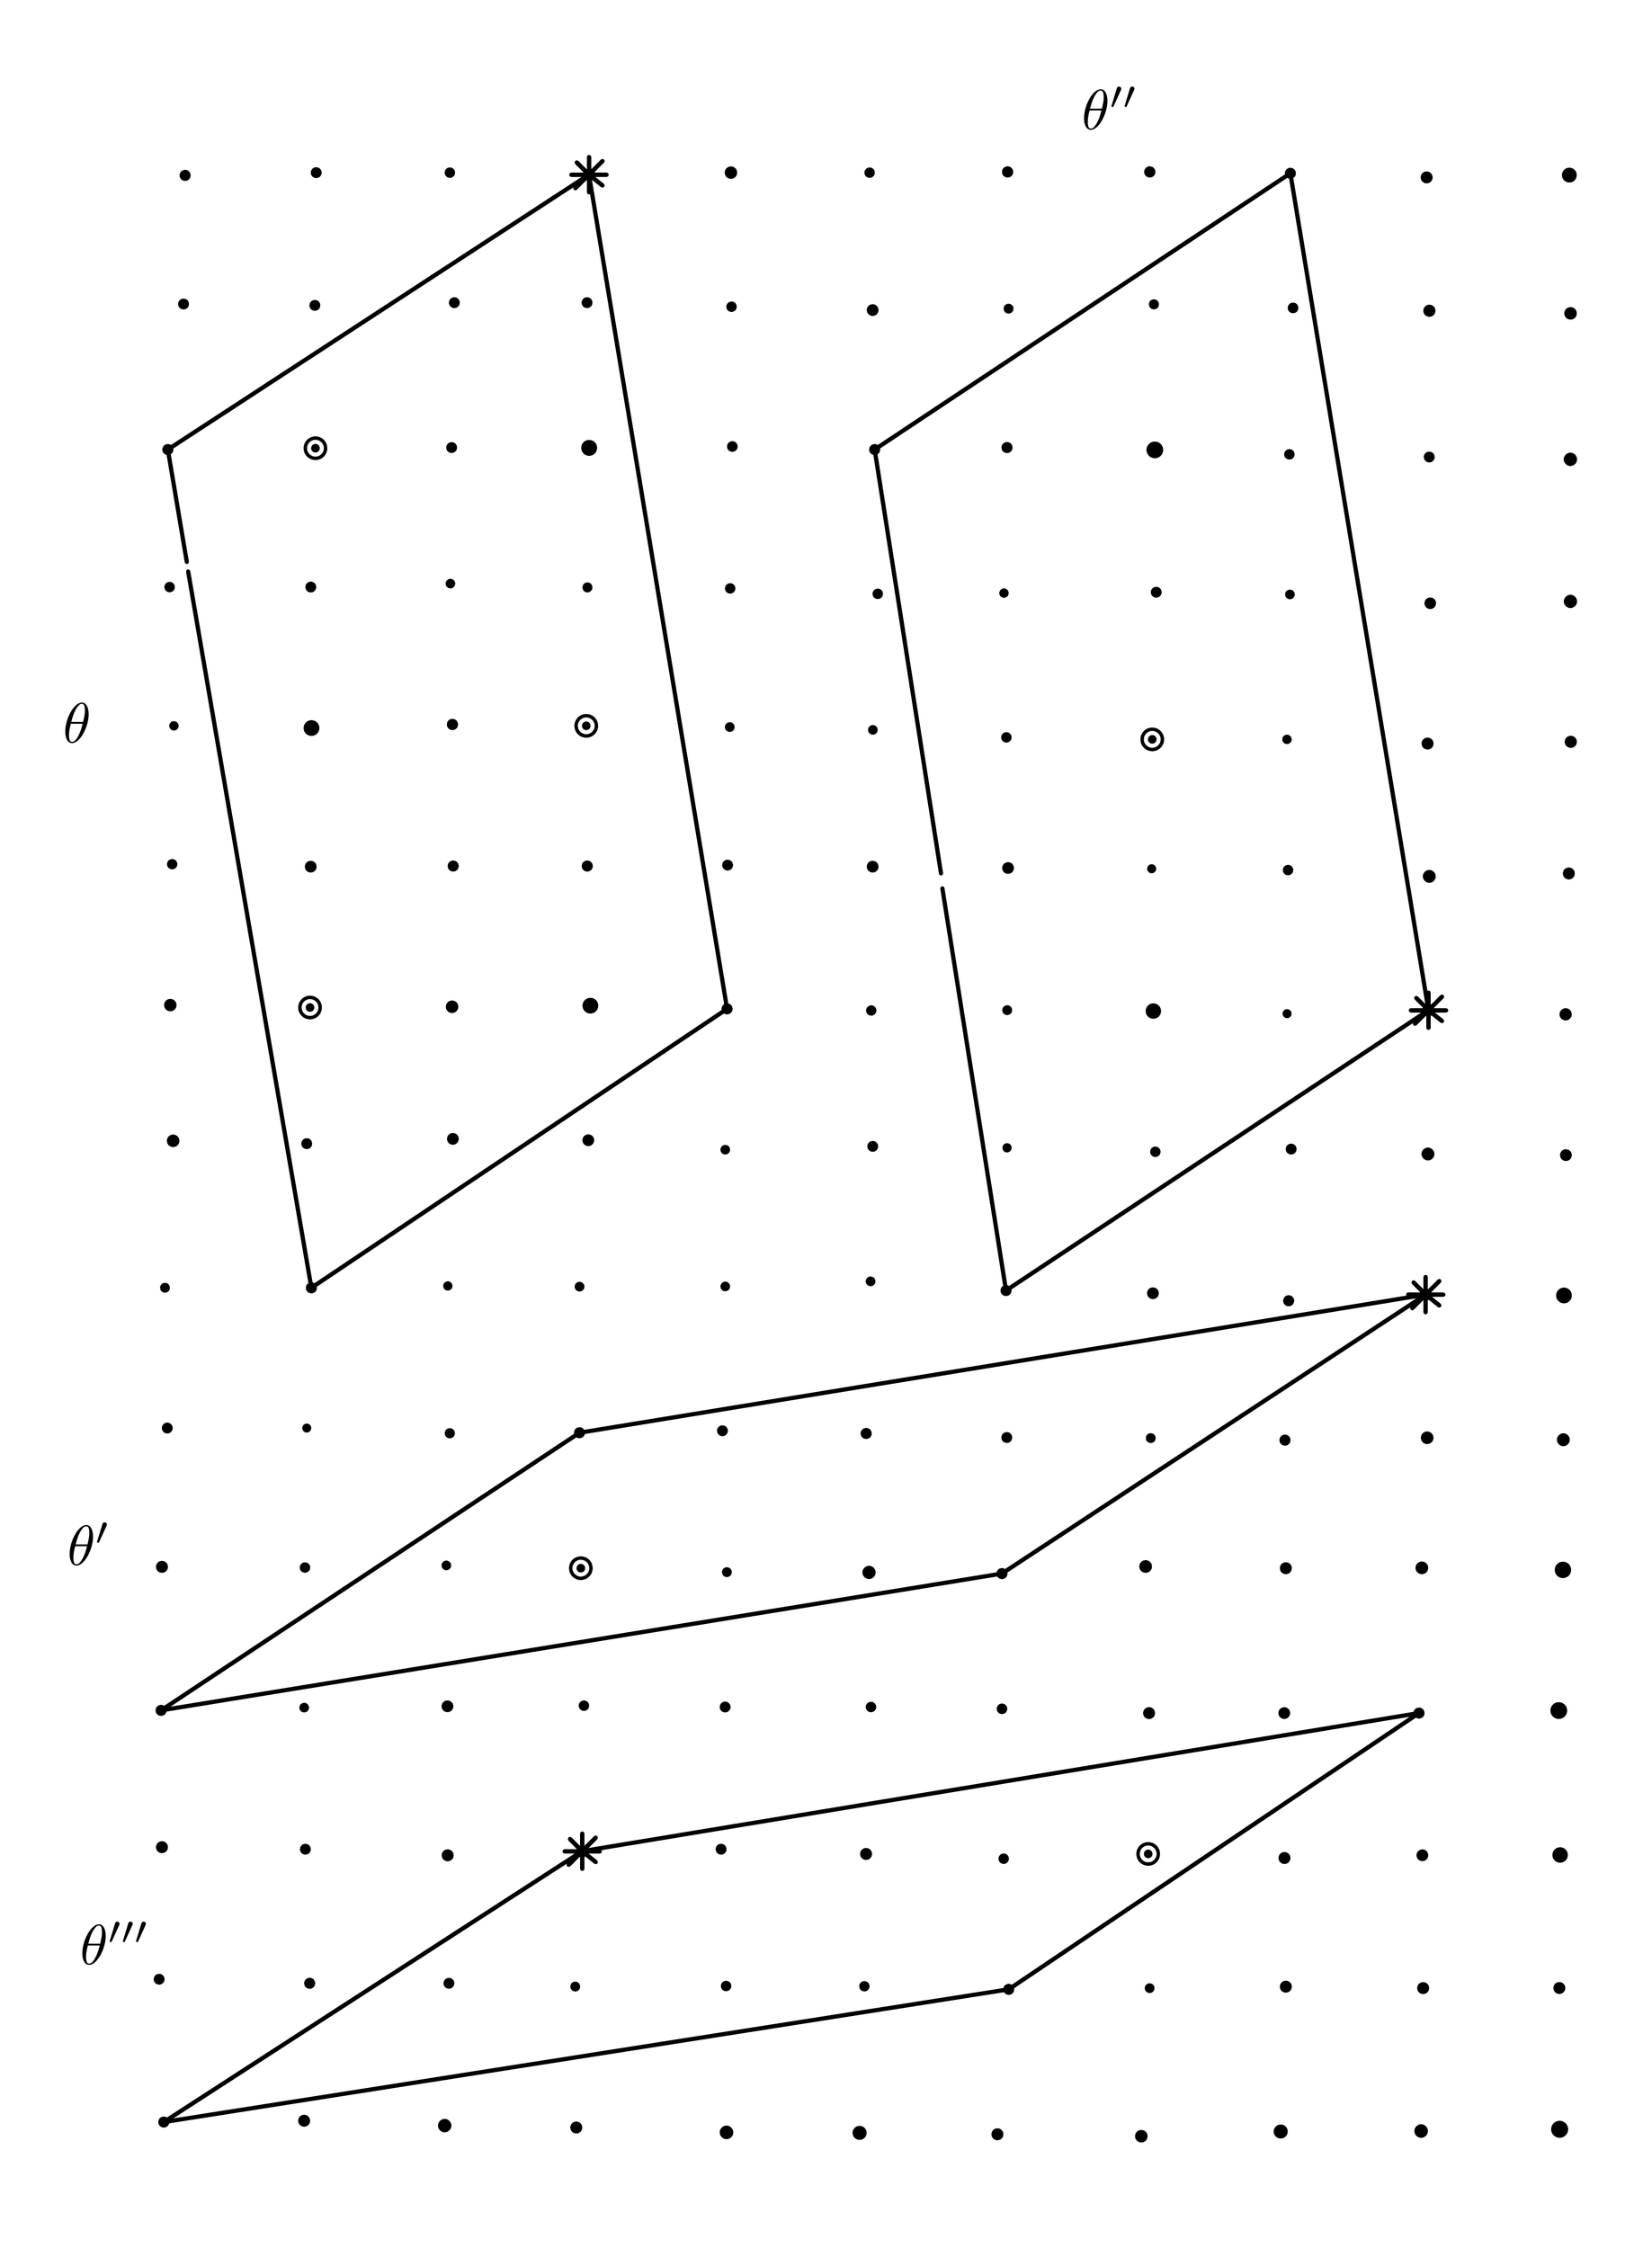
\begin{tikzpicture}[x=1bp,y=-1bp,line cap=round,line join=round]
\path[use as bounding box] (0,0) rectangle (1200,1640);
\begin{pgfinterruptboundingbox}
\draw[line width=3.1bp] (114,322) -- (425,119) -- (527,735) -- (220,941) -- (129,412);
\draw[line width=3.1bp] (128,405) -- (114,322);
\draw[line width=3.1bp] (636,322) -- (943,118) -- (1045,736) -- (733,943) -- (686,646);
\draw[line width=3.1bp] (685,635) -- (636,322);
\draw[line width=3.1bp] (109,1253) -- (418,1048) -- (1043,946) -- (730,1152) -- cycle;
\draw[line width=3.1bp] (111,1557) -- (420,1357) -- (1038,1255) -- (735,1459) -- cycle;
\fill (126.74,119.53) circle[radius=4.11bp];
\fill (223.57,117.53) circle[radius=4.03bp];
\fill (322.28,117.53) circle[radius=3.87bp];
\fill (425,119) circle[radius=4.5bp];
\draw[line width=3.2bp] (425,119) -- (425,106);
\draw[line width=3.2bp] (425,119) -- (435,109);
\draw[line width=3.2bp] (425,119) -- (438,119);
\draw[line width=3.2bp] (425,119) -- (435,127);
\draw[line width=3.2bp] (425,119) -- (425,132);
\draw[line width=3.2bp] (425,119) -- (415,129);
\draw[line width=3.2bp] (425,119) -- (412,119);
\draw[line width=3.2bp] (425,119) -- (416,110);
\fill (529.85,117.52) circle[radius=4.62bp];
\fill (632.28,117.53) circle[radius=3.87bp];
\fill (734.18,117.0) circle[radius=4.18bp];
\fill (839.18,117.0) circle[radius=4.18bp];
\fill (943,118) circle[radius=4.1bp];
\fill (1043.65,121.02) circle[radius=4.44bp];
\fill (1149.04,119.35) circle[radius=5.47bp];
\fill (125.57,214.53) circle[radius=4.03bp];
\fill (222.57,215.53) circle[radius=4.03bp];
\fill (325.57,213.53) circle[radius=4.03bp];
\fill (423.57,213.53) circle[radius=4.03bp];
\fill (530.28,216.53) circle[radius=3.87bp];
\fill (634.5,219.0) circle[radius=4.37bp];
\fill (734.88,217.95) circle[radius=3.66bp];
\fill (842.23,214.77) circle[radius=3.74bp];
\fill (944.98,217.41) circle[radius=3.95bp];
\fill (1045.66,219.5) circle[radius=4.51bp];
\fill (1149.91,221.44) circle[radius=4.65bp];
\fill (114,322) circle[radius=4.1bp];
\fill (223,321) circle[radius=3.2bp];
\draw[line width=2.5bp] (223,321) circle[radius=7.5bp];
\fill (323.57,320.53) circle[radius=4.03bp];
\fill (425.14,320.75) circle[radius=5.86bp];
\fill (530.88,319.73) circle[radius=3.95bp];
\fill (636,322) circle[radius=4.1bp];
\fill (733.74,320.53) circle[radius=4.11bp];
\fill (842.9,322.25) circle[radius=6.15bp];
\fill (942.28,325.53) circle[radius=3.87bp];
\fill (1045.57,327.53) circle[radius=4.03bp];
\fill (1149.8,329.21) circle[radius=4.92bp];
\fill (115.28,423.53) circle[radius=3.87bp];
\fill (219.57,423.53) circle[radius=4.03bp];
\fill (322.68,420.98) circle[radius=3.57bp];
\fill (423.88,423.79) circle[radius=3.7bp];
\fill (529.28,424.53) circle[radius=3.87bp];
\fill (638.28,428.53) circle[radius=3.87bp];
\fill (731.5,428.0) circle[radius=3.48bp];
\fill (843.94,427.35) circle[radius=4.03bp];
\fill (942.68,428.98) circle[radius=3.57bp];
\fill (1046.31,435.5) circle[radius=4.3bp];
\fill (1149.84,434.13) circle[radius=4.89bp];
\fill (118.5,526.0) circle[radius=3.48bp];
\fill (220.06,527.64) circle[radius=5.81bp];
\fill (324.18,525.0) circle[radius=4.18bp];
\fill (423,526) circle[radius=3.2bp];
\draw[line width=2.5bp] (423,526) circle[radius=7.5bp];
\fill (528.98,526.88) circle[radius=3.61bp];
\fill (634.67,528.98) circle[radius=3.57bp];
\fill (733.28,534.53) circle[radius=3.87bp];
\fill (841,536) circle[radius=3.2bp];
\draw[line width=2.5bp] (841,536) circle[radius=7.5bp];
\fill (940.5,536.0) circle[radius=3.48bp];
\fill (1044.31,539.1) circle[radius=4.44bp];
\fill (1150.09,537.81) circle[radius=4.51bp];
\fill (117.2,628.17) circle[radius=3.83bp];
\fill (219.5,630.0) circle[radius=4.37bp];
\fill (324.74,629.53) circle[radius=4.11bp];
\fill (423.74,629.53) circle[radius=4.11bp];
\fill (527.39,628.84) circle[radius=4.03bp];
\fill (634.5,630.0) circle[radius=4.37bp];
\fill (734.5,631.0) circle[radius=4.37bp];
\fill (840.57,631.54) circle[radius=3.34bp];
\fill (941.28,632.53) circle[radius=3.87bp];
\fill (1045.61,637.17) circle[radius=4.75bp];
\fill (1148.65,635.02) circle[radius=4.44bp];
\fill (115.82,732.21) circle[radius=4.62bp];
\fill (219,734) circle[radius=3.2bp];
\draw[line width=2.5bp] (219,734) circle[radius=7.5bp];
\fill (323.91,733.44) circle[radius=4.65bp];
\fill (426.06,732.64) circle[radius=5.81bp];
\fill (527,735) circle[radius=4.1bp];
\fill (633.46,736.2) circle[radius=3.83bp];
\fill (733.88,735.95) circle[radius=3.66bp];
\fill (841.81,736.62) circle[radius=5.67bp];
\fill (940.57,738.54) circle[radius=3.34bp];
\fill (1045,736) circle[radius=4.5bp];
\draw[line width=3.2bp] (1045,736) -- (1045,723);
\draw[line width=3.2bp] (1045,736) -- (1055,726);
\draw[line width=3.2bp] (1045,736) -- (1058,736);
\draw[line width=3.2bp] (1045,736) -- (1055,744);
\draw[line width=3.2bp] (1045,736) -- (1045,749);
\draw[line width=3.2bp] (1045,736) -- (1035,746);
\draw[line width=3.2bp] (1045,736) -- (1032,736);
\draw[line width=3.2bp] (1045,736) -- (1036,727);
\fill (1146.29,739.03) circle[radius=4.55bp];
\fill (117.91,832.44) circle[radius=4.65bp];
\fill (216.57,834.53) circle[radius=4.03bp];
\fill (324.5,831.0) circle[radius=4.37bp];
\fill (424.5,832.0) circle[radius=4.37bp];
\fill (525.67,838.98) circle[radius=3.57bp];
\fill (634.57,836.53) circle[radius=4.03bp];
\fill (733.76,837.59) circle[radius=3.43bp];
\fill (843.28,840.53) circle[radius=3.87bp];
\fill (943.57,838.53) circle[radius=4.03bp];
\fill (1044.61,842.17) circle[radius=4.75bp];
\fill (1146.5,843.0) circle[radius=4.37bp];
\fill (111.88,940.95) circle[radius=3.66bp];
\fill (220,941) circle[radius=4.1bp];
\fill (320.76,939.59) circle[radius=3.43bp];
\fill (418.05,940.12) circle[radius=3.61bp];
\fill (525.67,939.98) circle[radius=3.57bp];
\fill (632.98,936.2) circle[radius=3.61bp];
\fill (733,943) circle[radius=4.1bp];
\fill (841.5,945.0) circle[radius=4.37bp];
\fill (941.74,950.53) circle[radius=4.11bp];
\fill (1043,946) circle[radius=4.5bp];
\draw[line width=3.2bp] (1043,946) -- (1043,933);
\draw[line width=3.2bp] (1043,946) -- (1053,936);
\draw[line width=3.2bp] (1043,946) -- (1056,946);
\draw[line width=3.2bp] (1043,946) -- (1053,954);
\draw[line width=3.2bp] (1043,946) -- (1043,959);
\draw[line width=3.2bp] (1043,946) -- (1033,956);
\draw[line width=3.2bp] (1043,946) -- (1030,946);
\draw[line width=3.2bp] (1043,946) -- (1034,937);
\fill (1145.06,946.64) circle[radius=5.81bp];
\fill (113.57,1044.53) circle[radius=4.03bp];
\fill (216.57,1044.54) circle[radius=3.34bp];
\fill (322.22,1048.38) circle[radius=3.78bp];
\fill (418,1048) circle[radius=4.1bp];
\fill (523.57,1046.53) circle[radius=4.03bp];
\fill (629.74,1048.53) circle[radius=4.11bp];
\fill (733.57,1051.53) circle[radius=4.03bp];
\fill (839.88,1051.95) circle[radius=3.66bp];
\fill (939.02,1053.45) circle[radius=4.11bp];
\fill (1044.03,1051.71) circle[radius=4.69bp];
\fill (1144.61,1053.17) circle[radius=4.75bp];
\fill (109.65,1147.02) circle[radius=4.44bp];
\fill (215.28,1147.53) circle[radius=3.87bp];
\fill (319.68,1145.97) circle[radius=3.57bp];
\fill (419,1148) circle[radius=3.2bp];
\draw[line width=2.5bp] (419,1148) circle[radius=7.5bp];
\fill (526.88,1150.95) circle[radius=3.66bp];
\fill (631.84,1151.13) circle[radius=4.89bp];
\fill (730,1152) circle[radius=4.1bp];
\fill (836.11,1146.76) circle[radius=4.72bp];
\fill (939.65,1148.02) circle[radius=4.44bp];
\fill (1040.11,1147.76) circle[radius=4.72bp];
\fill (1144.3,1149.26) circle[radius=6.05bp];
\fill (109,1253) circle[radius=4.1bp];
\fill (214.68,1250.97) circle[radius=3.57bp];
\fill (320.5,1250.0) circle[radius=4.37bp];
\fill (421.28,1249.53) circle[radius=3.87bp];
\fill (525.57,1250.53) circle[radius=4.03bp];
\fill (633.28,1250.53) circle[radius=3.87bp];
\fill (730.02,1251.85) circle[radius=3.91bp];
\fill (838.65,1255.02) circle[radius=4.44bp];
\fill (938.5,1255.0) circle[radius=4.37bp];
\fill (1038,1255) circle[radius=4.1bp];
\fill (1141.22,1253.14) circle[radius=6.18bp];
\fill (109.65,1354.02) circle[radius=4.44bp];
\fill (215.57,1355.53) circle[radius=4.03bp];
\fill (320.65,1360.02) circle[radius=4.44bp];
\fill (420,1357) circle[radius=4.5bp];
\draw[line width=3.2bp] (420,1357) -- (420,1344);
\draw[line width=3.2bp] (420,1357) -- (430,1347);
\draw[line width=3.2bp] (420,1357) -- (433,1357);
\draw[line width=3.2bp] (420,1357) -- (430,1365);
\draw[line width=3.2bp] (420,1357) -- (420,1370);
\draw[line width=3.2bp] (420,1357) -- (410,1367);
\draw[line width=3.2bp] (420,1357) -- (407,1357);
\draw[line width=3.2bp] (420,1357) -- (411,1348);
\fill (522.57,1355.53) circle[radius=4.03bp];
\fill (629.65,1359.02) circle[radius=4.44bp];
\fill (731.28,1362.53) circle[radius=3.87bp];
\fill (838,1359) circle[radius=3.2bp];
\draw[line width=2.5bp] (838,1359) circle[radius=7.5bp];
\fill (938.65,1362.02) circle[radius=4.44bp];
\fill (1040.5,1360.0) circle[radius=4.37bp];
\fill (1142.22,1359.78) circle[radius=5.7bp];
\fill (107.57,1451.53) circle[radius=4.03bp];
\fill (218.74,1454.53) circle[radius=4.11bp];
\fill (321.57,1454.53) circle[radius=4.03bp];
\fill (414.88,1456.95) circle[radius=3.66bp];
\fill (526.28,1456.53) circle[radius=3.87bp];
\fill (628.41,1456.72) circle[radius=3.83bp];
\fill (735,1459) circle[radius=4.1bp];
\fill (839.05,1458.12) circle[radius=3.61bp];
\fill (939.65,1457.02) circle[radius=4.44bp];
\fill (1041.06,1458.08) circle[radius=4.44bp];
\fill (1141.65,1458.02) circle[radius=4.44bp];
\fill (111,1557) circle[radius=4.1bp];
\fill (214.65,1556.02) circle[radius=4.44bp];
\fill (318.44,1559.62) circle[radius=4.95bp];
\fill (415.65,1561.02) circle[radius=4.44bp];
\fill (526.58,1564.62) circle[radius=5.01bp];
\fill (624.87,1564.98) circle[radius=5.17bp];
\fill (726.65,1566.02) circle[radius=4.44bp];
\fill (832.91,1567.44) circle[radius=4.65bp];
\fill (935.87,1563.98) circle[radius=5.17bp];
\fill (1039.58,1563.62) circle[radius=5.01bp];
\fill (1141.86,1562.33) circle[radius=6.26bp];
\node[inner sep=0pt,outer sep=0pt,anchor=center] at (47,524) {\scalebox{4.2}{\ensuremath{\theta}}};
\node[inner sep=0pt,outer sep=0pt,anchor=center] at (56,1130) {\scalebox{4.2}{\ensuremath{\theta'}}};
\node[inner sep=0pt,outer sep=0pt,anchor=center] at (810,70) {\scalebox{4.2}{\ensuremath{\theta''}}};
\node[inner sep=0pt,outer sep=0pt,anchor=center] at (75,1425) {\scalebox{4.2}{\ensuremath{\theta'''}}};
\end{pgfinterruptboundingbox}
\end{tikzpicture}
}
\end{center}
